\documentclass[10pt,twocolumn,a4paper]{article}
\usepackage[margin=0.7in]{geometry}
\usepackage[T1]{fontenc}
\usepackage[utf8]{inputenc}
\usepackage{graphicx}
\usepackage{booktabs}
\usepackage{hyperref}
\usepackage{xcolor}

\hypersetup{
    colorlinks=true,
    linkcolor=blue,
    urlcolor=blue
}

\title{PostgreSQL-Backed Transport Analytics for Paris and New York City}
\author{Big Data Project}
\date{\today}

\begin{document}
\maketitle

\begin{abstract}
This project analyzes public-transport demand in Paris and New York City using
PostgreSQL as the single analytical source of truth. Source tables in the
\texttt{public} schema are exposed through reporting-clean views in the
\texttt{transport} schema, then consumed by a Python workflow that generates
reproducible result tables and figures. The final method set contains four
components: temporal profiling, lag-based forecasting, anomaly detection, and
contributor / city-structure comparison. On the current reporting scope, the
forecasting baseline achieves an overall mean absolute percentage error of
\(6.02\%\), with stronger performance for NYC (\(5.86\%\)) than Paris
(\(6.94\%\)). Paris shows a higher anomaly rate (\(8.96\%\)) than NYC
(\(0.73\%\)), while Paris also exhibits higher average daily demand
(\(\approx 4.13\) million) than NYC (\(\approx 2.63\) million).
\end{abstract}

\section{Introduction}

The goal of this project is to compare large-scale transport demand patterns in
Paris and New York City using one reproducible analytical workflow. Earlier
iterations of the repository mixed exploratory notebook material, local-file
assumptions, and placeholder narrative. The current baseline removes that
ambiguity: PostgreSQL stores the authoritative source data, SQL views define the
reporting contract, and Python produces the final derived outputs under
\texttt{report/results/}.

This report is written from the current generated outputs rather than from
earlier placeholder material. The emphasis is on defensible interpretation:
how demand evolves over time, how well a simple forecasting model performs,
which observations are anomalous, and which stations dominate total traffic.

\section{Data and Architecture}

The project reads three source datasets already loaded into PostgreSQL:

\begin{itemize}
\item \texttt{public.idfm\_daily\_validations} with station-level Paris daily validations,
\item \texttt{public.idfm\_hourly\_profiles} with Paris hourly validation shares,
\item \texttt{public.mta\_hourly\_ridership} with NYC hourly ridership.
\end{itemize}

Reference tables \texttt{public.idfm} and \texttt{public.mta} provide network
metadata. The analytical contract is defined in the \texttt{transport} schema:

\begin{itemize}
\item \texttt{v\_daily\_demand} for reporting-clean daily demand,
\item \texttt{v\_nyc\_hourly\_profile} and \texttt{v\_paris\_hourly\_profile},
\item \texttt{v\_contributor\_source} for station contribution ranking,
\item \texttt{v\_city\_structure\_source} for city-level comparison.
\end{itemize}

Incomplete boundary years are excluded from the reporting views, which removes
the partial Paris 2025 year from the final result set. The final workflow
contains \(12{,}696\) daily rows and \(2{,}003\) contributor rows in the
generated summary output.

\begin{figure}[t]
\centering
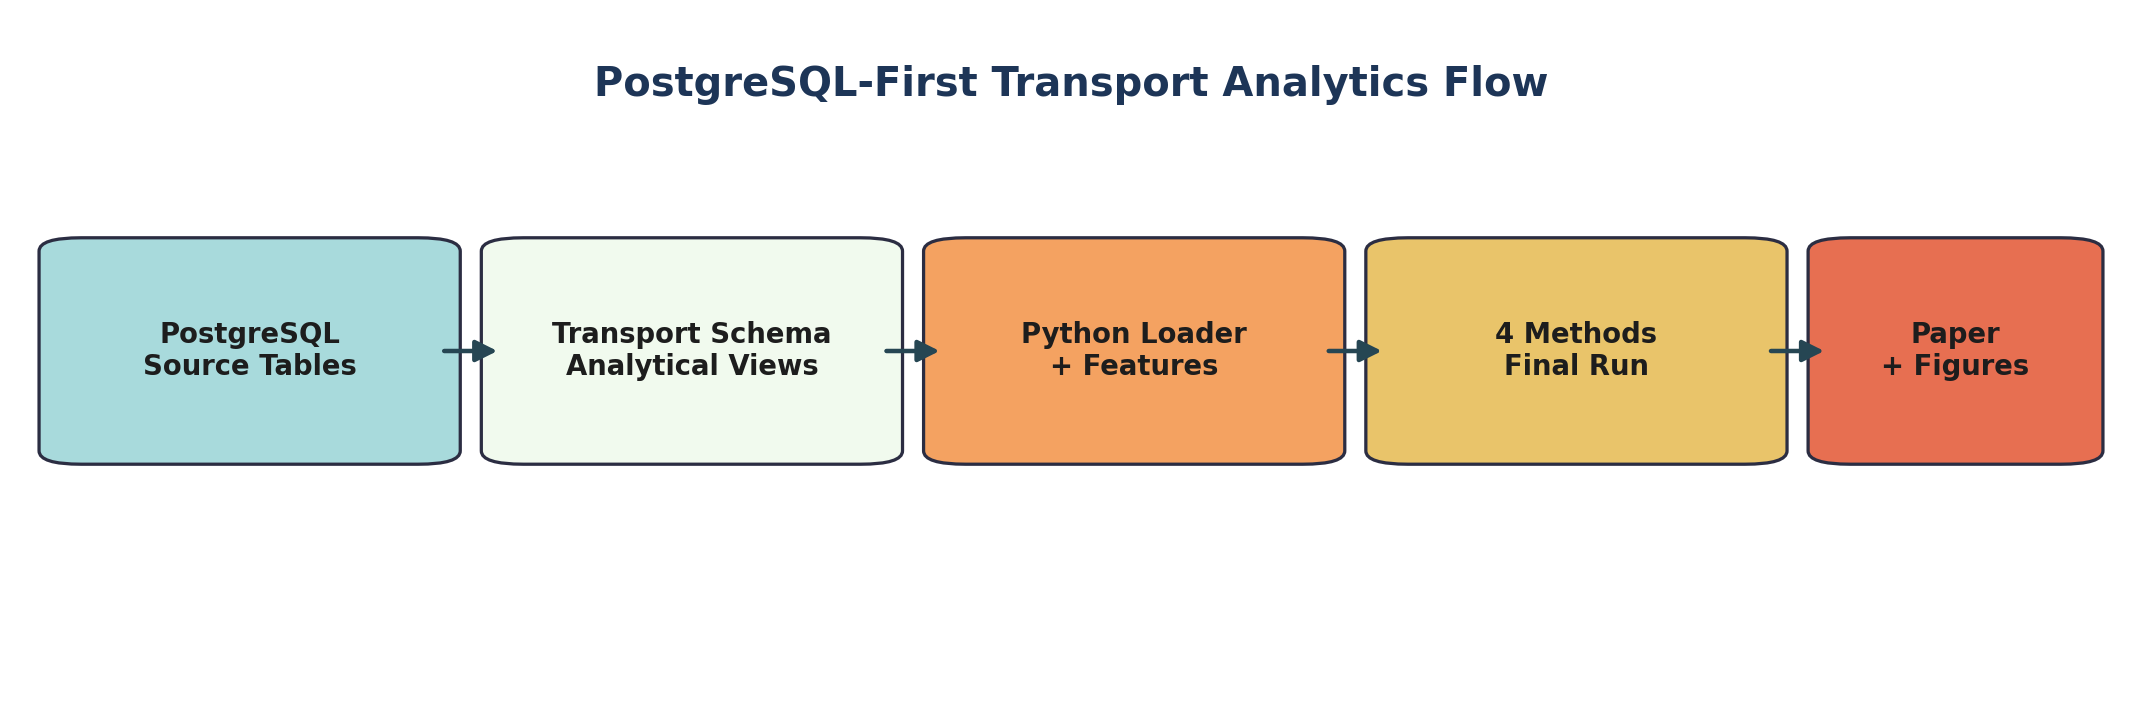
\includegraphics[width=\linewidth]{figures/workflow_diagram.png}
\caption{Final PostgreSQL-first analysis flow used by the project.}
\end{figure}

\section{Methods}

The final method set contains four components.

\textbf{Temporal profiling.} Daily demand is summarized by weekday, month, and
year, while hourly profiles are analyzed separately for NYC ridership and Paris
validation shares.

\textbf{Forecasting.} A lag-based random forest baseline uses lag features,
rolling statistics, and calendar features. The model is evaluated with a
time-ordered train/test split.

\textbf{Anomaly detection.} A hybrid rule combines rolling z-scores with an
\texttt{IsolationForest} model fitted on value and lag-derived features.

\textbf{Contributor and city-structure analysis.} Station-level demand is
ranked to identify dominant contributors, and city-level summaries are computed
for average daily demand, variability, seasonality, and weekend sensitivity.

\section{Results}

\subsection{Temporal patterns}

The yearly totals confirm the reporting-clean scope: NYC covers 2020--2024 and
Paris covers 2015--2024, with the partial 2025 year removed. Monthly structure
is visibly different across the two systems. NYC peaks in winter and early
autumn, while Paris peaks in October and weakens sharply in August.

\begin{figure}[t]
\centering
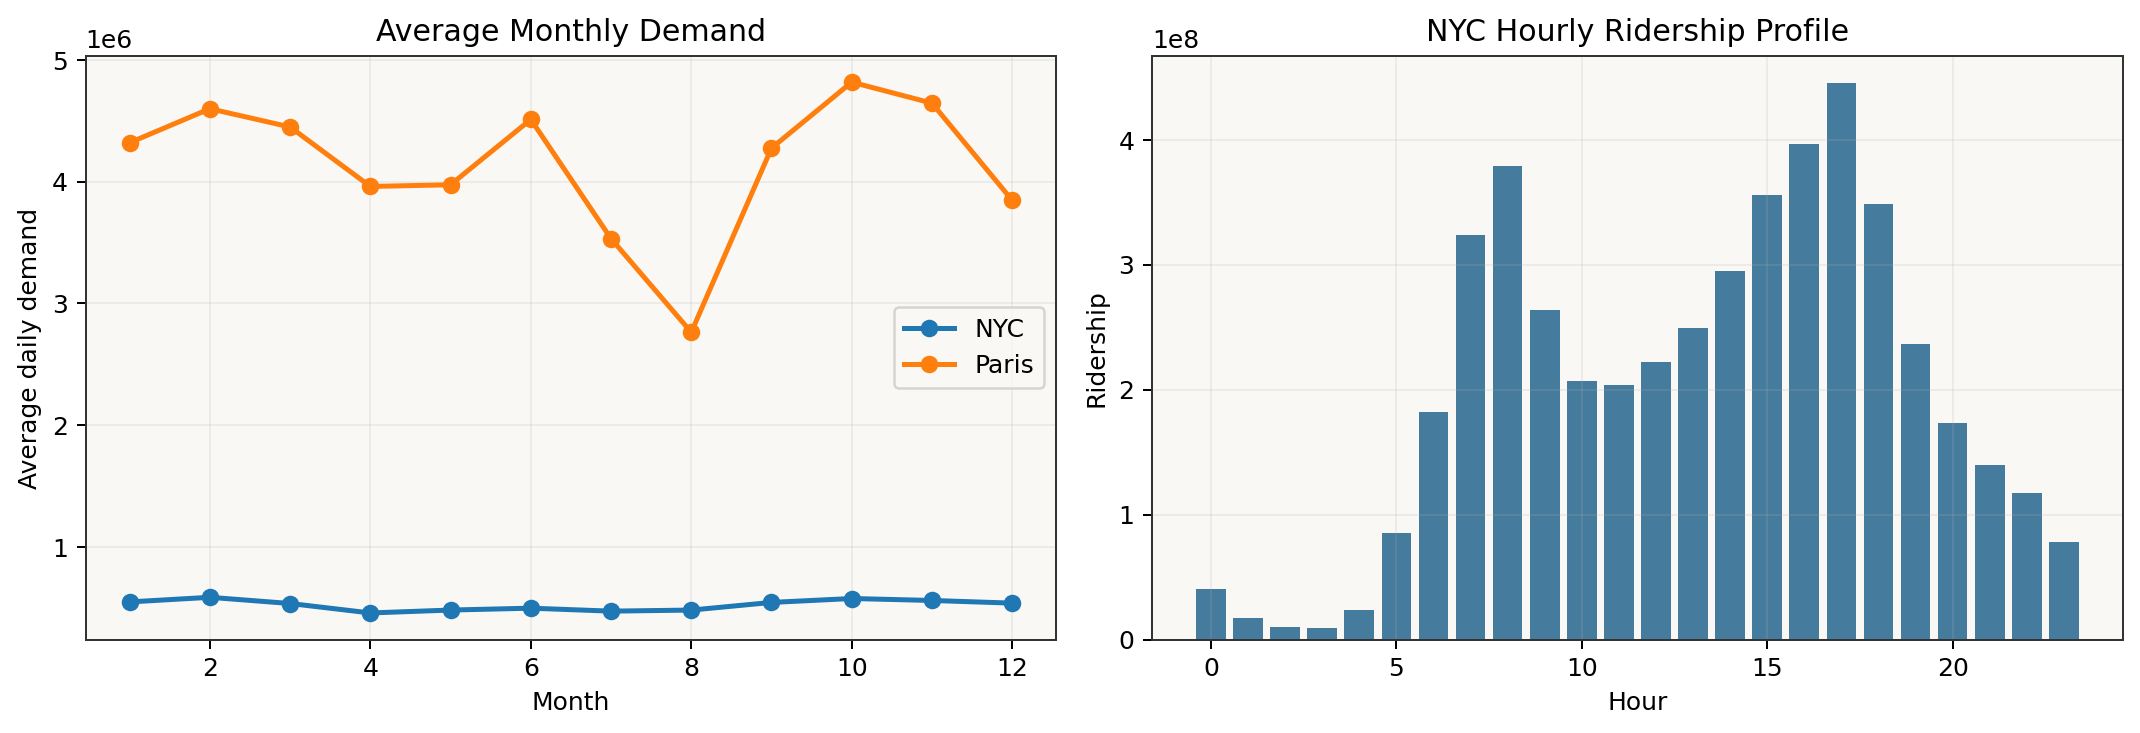
\includegraphics[width=\linewidth]{figures/temporal_profiles.png}
\caption{Monthly demand and NYC hourly ridership profile from the current run.}
\end{figure}

\subsection{Forecasting}

The forecasting baseline remains strong enough to support the final paper. The
overall model is trained on \(8{,}336\) rows and evaluated on \(4{,}276\) rows,
with an overall MAE of \(52{,}909\), RMSE of \(156{,}343\), and MAPE of
\(6.02\%\).

\begin{table}[t]
\centering
\caption{Forecast accuracy by city}
\begin{tabular}{lrrr}
\toprule
City & MAE & RMSE & MAPE \\
\midrule
NYC & 29,402 & 62,965 & 5.86\% \\
Paris & 187,446 & 376,361 & 6.94\% \\
\bottomrule
\end{tabular}
\end{table}

NYC forecasts are more stable in absolute terms, but both cities remain within
a single-digit MAPE range. This is sufficient for a baseline forecasting
section in the final report, although the Paris series is clearly harder to
predict due to larger swings and lower short-term regularity.

\begin{figure}[t]
\centering
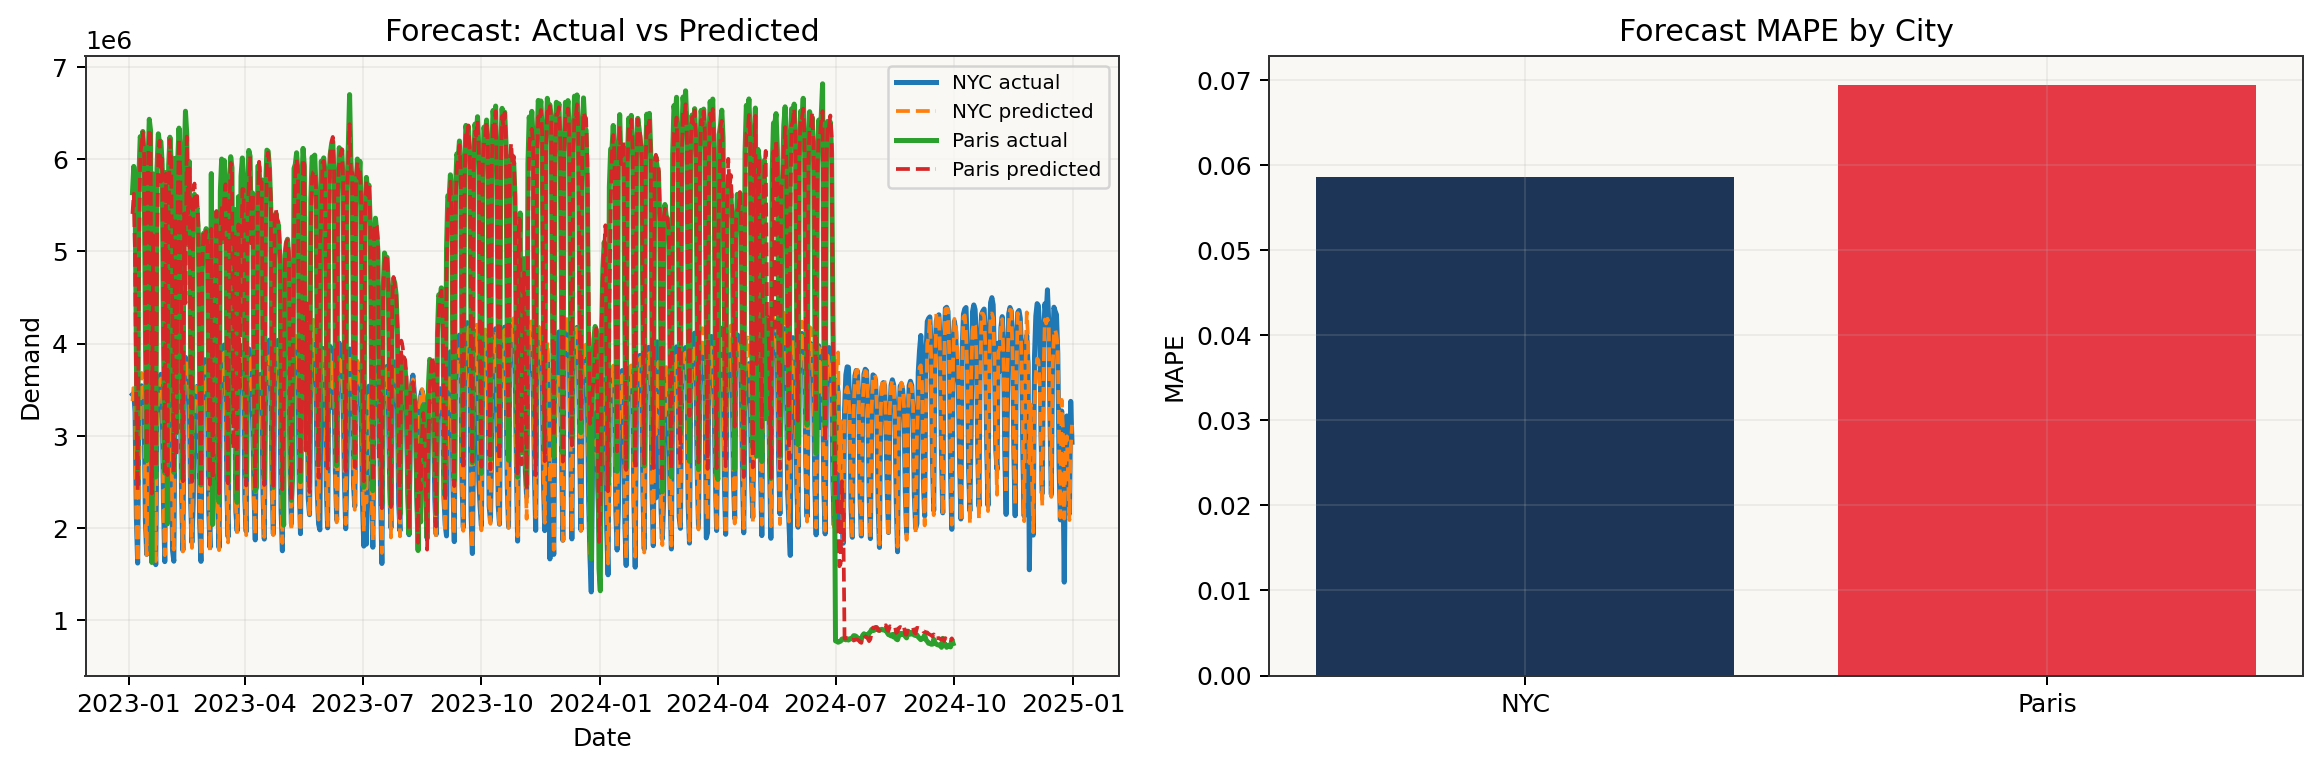
\includegraphics[width=\linewidth]{figures/forecast_performance.png}
\caption{Forecast quality from the current PostgreSQL-backed result set.}
\end{figure}

\subsection{Anomalies}

Anomaly rates remain highly asymmetric between the two cities. NYC has an
anomaly rate of \(0.73\%\), while Paris reaches \(8.96\%\). The largest Paris
anomalies cluster around 2020 disruption and recovery periods, whereas NYC
outliers are concentrated around holiday and unusually weak weekend traffic.

\subsection{Contributors and city structure}

Paris has the larger system-level demand in the current reporting scope. Its
average daily demand is approximately \(4.13\) million versus \(2.63\) million
for NYC. Paris also shows a lower weekend-to-weekday ratio (\(0.512\)) than NYC
(\(0.584\)), which indicates stronger weekday concentration.

\begin{table}[t]
\centering
\caption{City structure summary}
\begin{tabular}{lrrr}
\toprule
City & Avg daily & Weekend/weekday & Peak month \\
\midrule
NYC & 2.63M & 0.584 & 2 \\
Paris & 4.13M & 0.512 & 10 \\
\bottomrule
\end{tabular}
\end{table}

The top contributor table is plausible after label cleanup. Paris is dominated
by Saint-Lazare, La D\'efense--Grande Arche, Gare de Lyon, Gare du Nord, and
Montparnasse. NYC is led by Times Sq--42 St, Grand Central--42 St,
34 St--Herald Sq, and 14 St--Union Sq.

\begin{figure}[t]
\centering
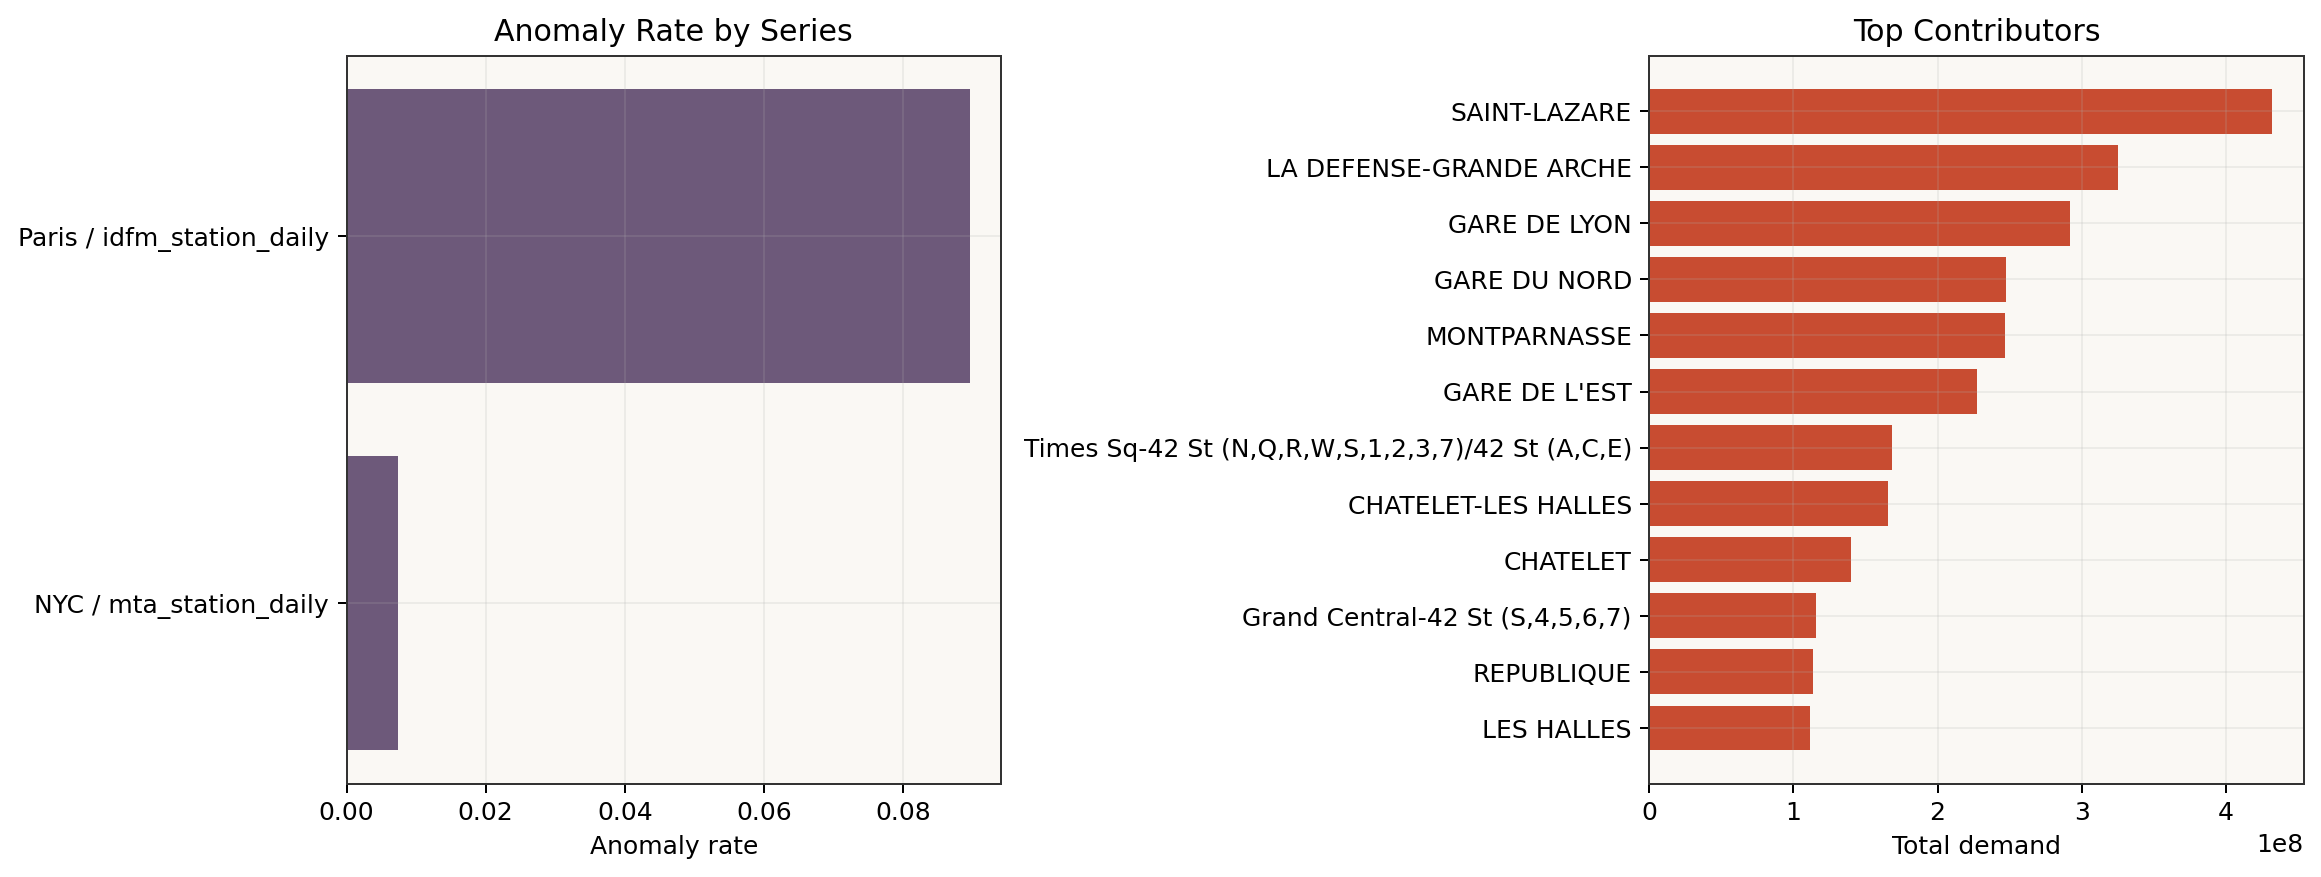
\includegraphics[width=\linewidth]{figures/anomalies_and_contributors.png}
\caption{Anomaly-rate contrast and top contributors in the cleaned result set.}
\end{figure}

\begin{figure}[t]
\centering
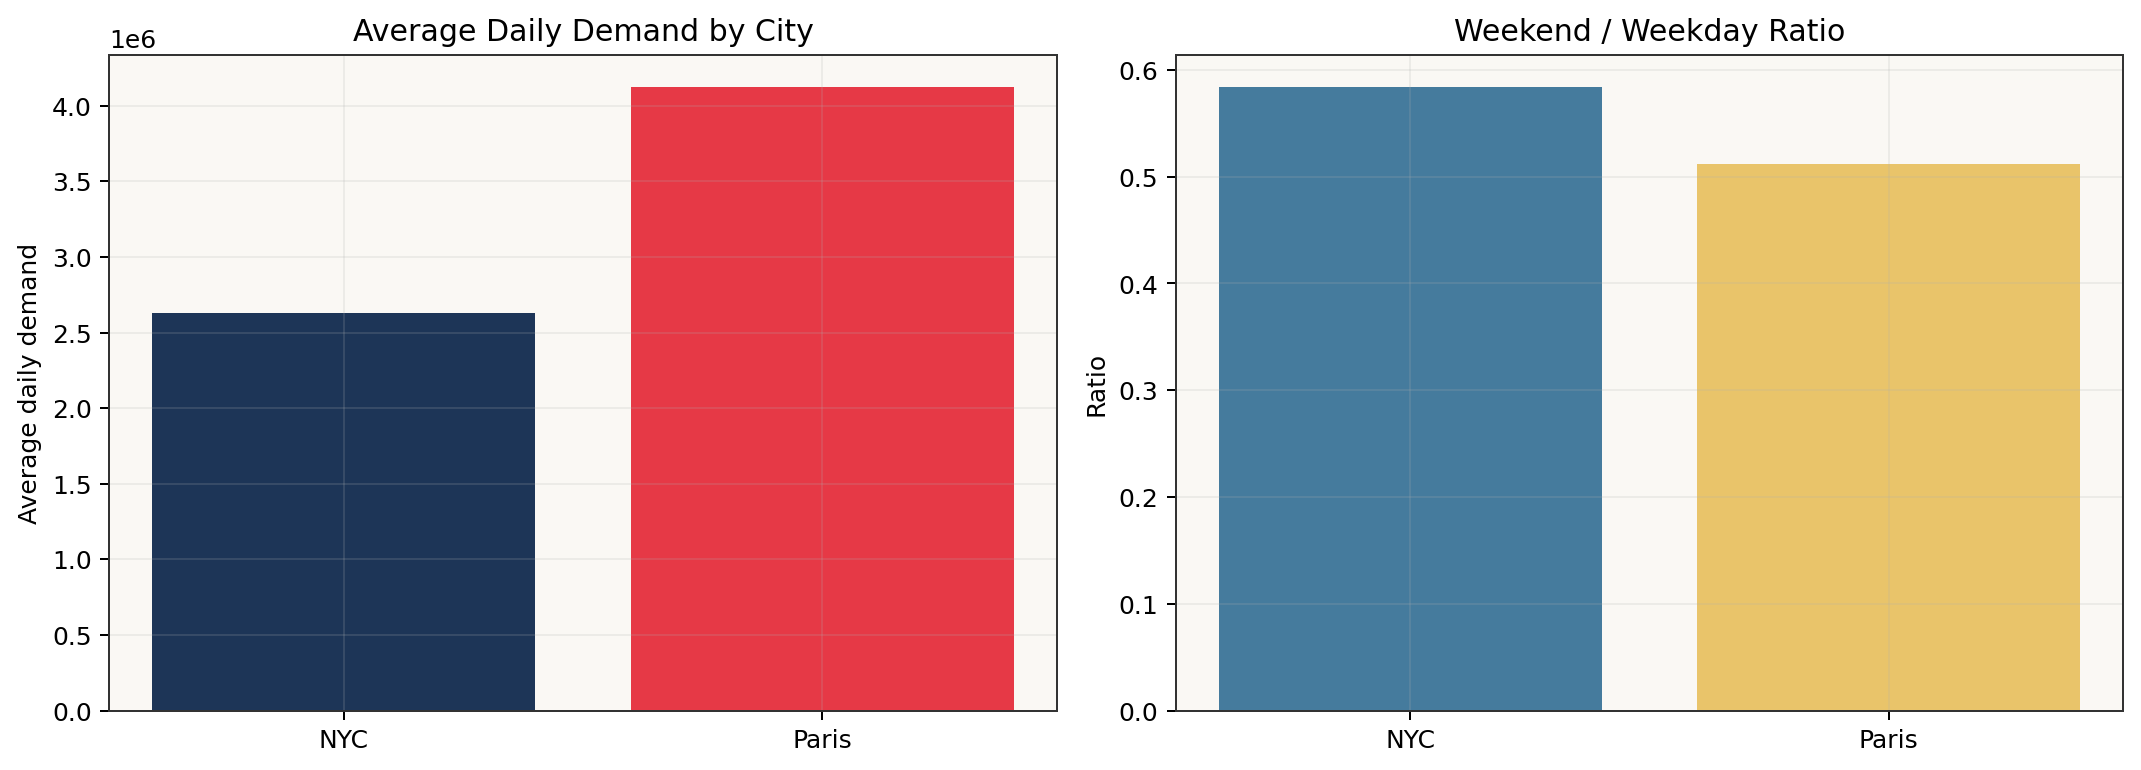
\includegraphics[width=\linewidth]{figures/city_structure.png}
\caption{Average daily demand and weekend sensitivity by city.}
\end{figure}

\section{Discussion and Limitations}

The project is now aligned around a reproducible database-backed workflow, but
several limitations remain.

First, the forecasting model is intentionally a baseline rather than a final
production forecaster. It captures broad structure well, but it does not model
special events, strikes, weather, or network interventions.

Second, the anomaly analysis is descriptive rather than causal. The flagged
observations indicate unusual behavior, but they do not prove why it happened.

Third, contributor ranking depends on the quality of station labeling in the
source tables. The obvious whitespace issues were removed during Stage 2
cleanup, but semantically similar stations are still treated as distinct when
their identifiers differ.

Finally, the notebook and report are derived from generated outputs rather than
from live database queries at compile time. That is acceptable for submission,
but it means the result regeneration step remains part of the reproducibility
contract.

\section{Conclusion}

The project now has a coherent final analytical baseline. PostgreSQL is the
single source of truth, the reporting views remove incomplete comparison years,
and the generated outputs support a defensible paper narrative. The main
findings are consistent across the final result set: Paris has higher overall
demand, stronger weekday concentration, and a much higher anomaly rate, while
NYC is easier to forecast with the current lag-based baseline. The repository is
now ready for final notebook alignment and submission cleanup rather than
another major analytical redesign.

\section*{References}

\begin{enumerate}
\item Project background papers stored under \texttt{docs/papers/}.
\item Generated analytical outputs stored under \texttt{report/results/}.
\item PostgreSQL analytical contract defined in \texttt{sql/02\_views.sql}.
\end{enumerate}

\end{document}
